\section{Dataset}
\label{sec:data}

A textual QA dataset with aspects is constructed for this aspect-based QA pairs generation task. 
SQuAD2.0 is a well known QA textual dataset with the amount of annotated QA pairs from documents.
Therefore in this paper, we just add the aspect keywords for each paragraph of the SQuAD2.0 dataset to support our experiments.

\subsection{Dataset Creation}
To allocate a suitable aspect keyword for each paragraph in SQuAD, we convert the paragraphs to original Wikipedia pages and extract the closest heading as the aspects.
In this step, to ensure that the paragraphs in SQuAD are consistent with the corresponding paragraphs in the original Wikipedia, 
we did not select wiki dumps as the source to obtain aspect keywords but crawled the most similar wiki texts which are distributed from between 2012 and 2016.

However, SQuAD only annotated a part of paragraphs from Wikipedia and there is a lack of ground truth QA of the unannotated paragraphs.
To make a suitable evaluation of our frameworks, we merge the paragraphs with annotated QA pairs as the input document $D$.
%Finally, we construct the dataset with the format $<$document, aspect keyword, paragraph, QA pairs$>$.

Figure \ref{fig:wiki} shows an example of a Wikipedia page with the information followed by the aspect-based QA dataset.

\begin{figure*}[th]
    \begin{center}
    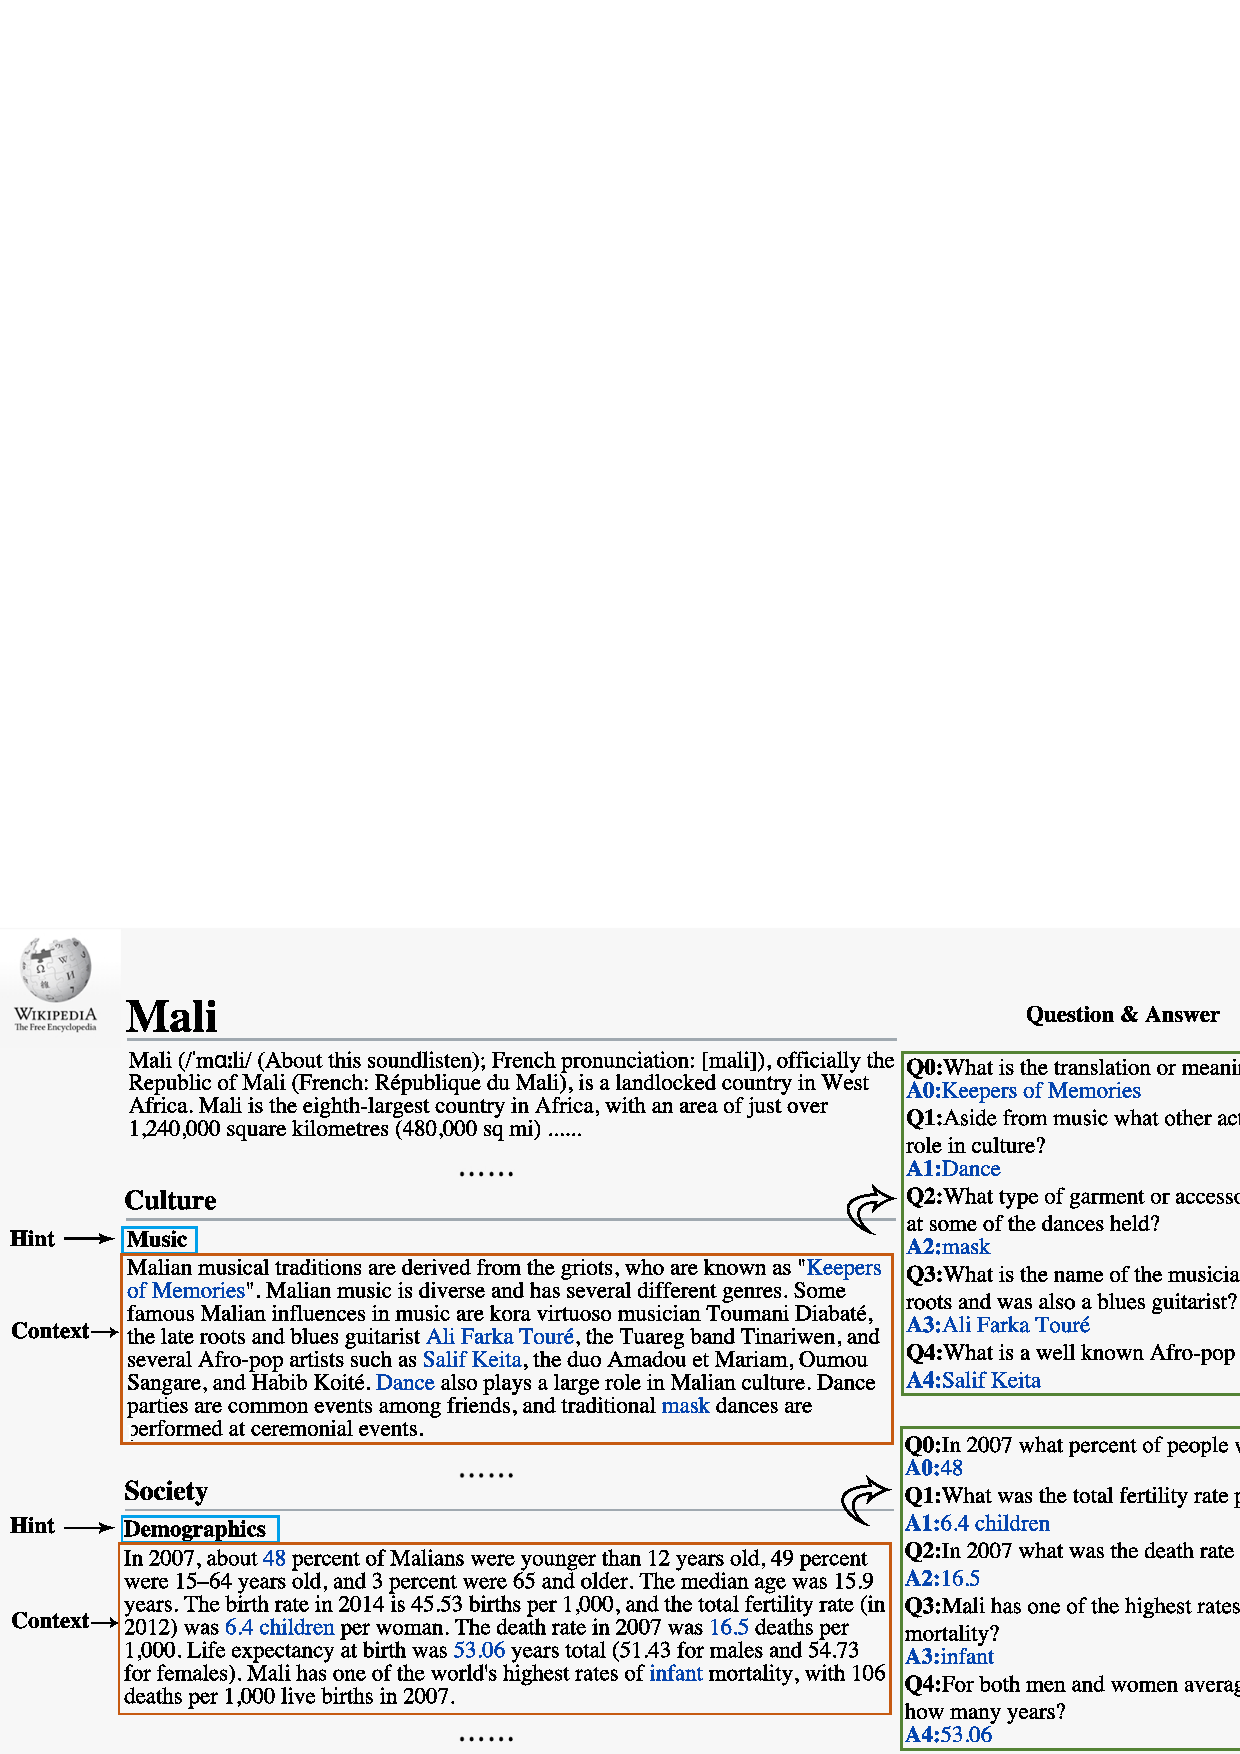
\includegraphics[width=0.8\textwidth]{pic/Wikipedia.pdf}
        \caption{\label{fig:wiki} An example of Wikipedia page \textbf{Black Death} and the information followed by our aspect-based QA dataset.
        The blocked context is the paragraph included in SQuAD2.0. The aspect keyword is the closest heading of the paragraph and the QA pairs on the right side are annotated in SQuAD2.0. The emoji in this figure is to show the relevance between the QA pairs and  aspect.}
    \end{center}
\end{figure*}

\subsection{Annotated Evaluation Set}
Although the paragraph is highly relevant to its aspect, not all of the QA pairs in SQuAD are related to this aspect.
The example in Figure \ref{fig:wiki} also shows this phenomenon. 
This paragraph talks about the causes of black death, in which QA1 and QA2 are relevant to this aspect.
However, QA0 is irrelevant which is talking about the details far from the topic.

We randomly select 100 QA pairs to judge whether they are relevant to their aspects, and find there are 60.58\% relevant samples.
Due to the noise in our dataset, there are two postgraduates asked to label the relevance between the hint and the QA pair.

We assume that noisy samples are still aspect useful.
To ensure sufficient training samples, we only manually select the relevant test data to do the evaluation.
%The labeled intersect positive samples are formed as the evaluation dataset.

\subsection{Size of the dataset}
Following the same data split method as Zhao et.al.~\shortcite{zhao2018paragraph},  we regard the dev* set as the test set, and split train set into train and dev sets randomly with the ratio of 9:1.
After adding the aspect words to each paragraph and manually labeling the QA pairs relevant to the corresponding aspects as the evaluation set, the size of our dataset is shown in Table \ref{tab:size}:
\begin{table}[th]
\scriptsize
\centering
\begin{tabular}{ccccc}
\hline
 & \textbf{\#Docs} & \textbf{\#Paragraphs} & \textbf{\#Aspects} & \textbf{\#QA pairs} \\ \hline
\textbf{train} & 398 & 17188 & 6421 & 78723 \\ 
\textbf{dev} & 44 & 1847 & 777 & 8098 \\ 
\textbf{annotation test} & 11 & 285 & 20 & 1018 \\ \hline
\end{tabular}
\caption{\label{tab:size} Size of our aspect-based dataset.}
\end{table}
